% 相反数的定义及函数图象
\begin{frame}{1.2 数轴}
\begin{definition}
\textbf{\textcolor{orange}{规定了原点、正方向和单位长度的直线叫做数轴(number axis).} } \\
\end{definition}
\vspace{12pt}
\textbf{数轴的四要素:} 
\begin{enumerate}[label={\arabic*.}]
    \item \textbf{原点}
    \item \textbf{正方向}
    \item \textbf{单位长度}
    \item \textbf{直线(强调三要素的只包括前三条)}
\end{enumerate}
\vspace{12pt}
\textbf{\textcolor{blue} {数轴示例:}}
\vspace{12pt}
\begin{figure}
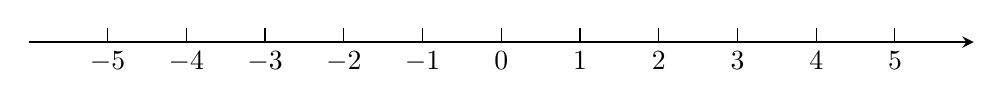
\begin{tikzpicture}
\draw [black, thick, ->, >=stealth] (-6,0) -- (6,0); 
\foreach \x in {-5, ..., 5}
	\draw (\x cm,5pt) -- (\x cm,0pt) node[anchor=north] {$\x$};
\end{tikzpicture}
\end{figure}
\end{frame}

\begin{frame}{1.2 数轴}
\begin{definition}
\textbf{\textcolor{orange}{规定了原点、正方向和单位长度的直线叫做数轴(number axis).} } \\
\end{definition}
\vspace{12pt}
\vspace{1cm}
\textbf{以下图形是不是一个数轴?:}
\vspace{1cm}
\begin{figure}
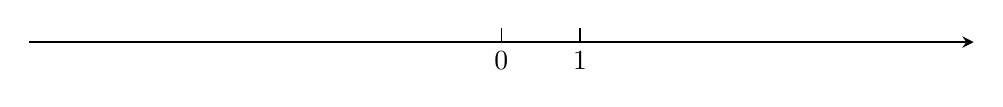
\begin{tikzpicture}
\draw [black, thick, ->, >=stealth] (-6,0) -- (6,0); 
\foreach \x in {0, 1}
 	\draw (\x cm,5pt) -- (\x cm,0pt) node[anchor=north] {$\x$};
\end{tikzpicture} 
\end{figure}
\end{frame}